\documentclass[fleqn,utf8,aspectratio=169,14pt]{beamer}
%\documentclass[fleqn,utf8,aspectratio=169,14pt,handout]{beamer}

\usepackage{url}
\usepackage{tabto}
\usepackage{dutchcal}
\usepackage{setspace}
\usepackage{xfrac}
\usefonttheme{serif}
\usepackage{graphicx}

\title{Tutorial do VSCode}
\author{Python para Todos}
\date{\today}

\graphicspath{{./figs/}}
\makeatletter
\def\input@path{{./figs/}}
\makeatother

\newcommand{\AddTeXFigure}[2]
{
	\begin{frame}{#1}
		\null
		\vspace*{-5mm}
		\hspace*{-10mm}
		\input{#2}
	\end{frame}
}
\begin{document}
	

	\begin{frame}
		\titlepage
	\end{frame}
	

	\begin{frame}{Sumário}
		\tableofcontents
	\end{frame}
	

	\section{Introdução}
	\begin{frame}{Introdução}
		O Visual Studio Code (VSCode) é um editor de código gratuito da Microsoft, rápido e personalizável, com:
		\begin{itemize}
			\item Destaque de sintaxe e autocompletar
			\item Extensões para várias linguagens (Python, JavaScript, etc.)
			\item Suporte a Git
			\item Interface moderna
		\end{itemize}
		Ideal para programadores de todos os níveis.
	\end{frame}
	
	\section{Como definir o tipo de um arquivo?}
	\begin{frame}{Como definir o tipo de um arquivo?}
		Para fazer isso no VSCode basta após inserir o nome do arquivo digitar "." seguido do seu tipo.\\
		Exemplo com o arquivo de nome "teste" em Python:\\
		
			\centering  Nome do arquivo: teste.py
	\end{frame}

	\section{Criando um arquivo}
	\begin{frame}{Criando um arquivo}
		Primeiro passo:
		Clicar em "File", no canto superior esquerdo, e em seguida em "New File ..."
		\centering 
		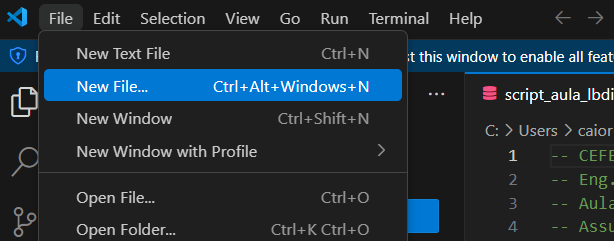
\includegraphics[width=0.8\textwidth]{Imagem1.png}
	\end{frame}
	
	\begin{frame}{Criando um arquivo}
		Segundo passo:
		Definir o nome do arquivo como "teste.py"
		\centering % Centraliza a imagem
		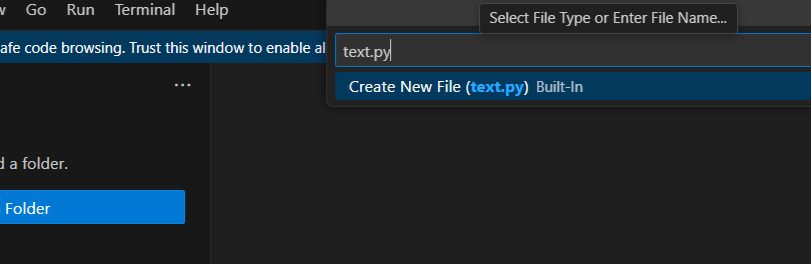
\includegraphics[width=0.8\textwidth]{Imagem2.png}
	\end{frame}
	
	\section{Executando o arquivo}
	\begin{frame}{Executando o arquivo}
		Digitar print("Hello World!")
		E em seguida vamos executar o código, clicando em Run Python File, no canto superior direito
		\centering % Centraliza a imagem
		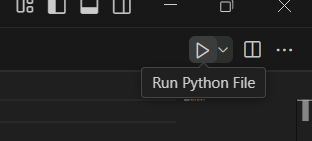
\includegraphics[width=0.8\textwidth]{Imagem3.png}
	\end{frame}
	
	
	\begin{frame}{Executando o arquivo}
		\centering % Centraliza a imagem
		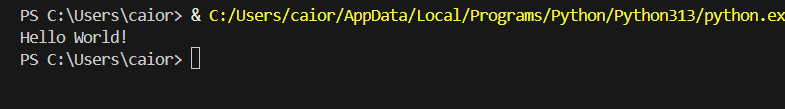
\includegraphics[width=1.2\textwidth]{Imagem4.png}
	\end{frame}
	
\end{document}}